%---------------------------Area-----------------------------
\section{Area\label{s:quad-area}}

Signed area, defined as
\[
q = \frac {1} {4} \sum_{i=0}^3 \alpha_i
\]
is useful for two purposes: first, the sign can indicate elements
that have vertices ordered incorrectly or arranged in a concave
pattern; and second, the magnitude can be used to identify
elements that are too small for accurate analysis.
Figure~\ref{f:quad-areas} shows how each vertex area contributes to
the total area of a quadrilateral.

\begin{figure}[htb]
  \centering
  \includegraphics[width=2in]{quad-areas}
  \caption{The areas associated with each vertex may be summed and
           weighted to get the area of the entire quadrilateral.%
                                                                  \label{f:quad-areas}}
\end{figure}

\quadmetrictable{area}%
{$L^2$}%                                    Dimension
{$[0,DBL\_MAX]$}%                           Acceptable range
{$[0,DBL\_MAX]$}%                           Normal range
{$[-DBL\_MAX,DBL\_MAX]$}%                   Full range
{$1$}%                                      Unit square
{--}%                                       Citation
{v\_quad\_area}%                            Verdict function name

